% http://www.idsc.ethz.ch/education/theses-semester-projects.html
% IDSC LaTeX Thesis Template
% 
% Author(s):	Eric Müller
% 				Institute for Dynamic Systems and Control
% 				Swiss Federal Institute of Technology (ETH) Zurich
% 
% Created:		2004/04/02  (Eric Mueller)
% 
% Notes: Has been tested on Windows 7 + MikTeX + TeXnicCenter
%
% Revisions: 	2009/05/29  (Soren Ebbesen)
% 				    2011/03/22	(Soren Ebbesen)
%             2013/03/08	(Soren Ebbesen)
%             2014/03/13	(Soren Ebbesen)
% ______________________________________________________________________________
\documentclass[11pt,twoside,a4paper,fleqn]{report}

\usepackage[english,mt]{ethidsc} % Special IDSC styles and commands      	
								 % {german}/english: language of headings, etc.
								 % {st}/bt/mt: {semester}/bachelor/master thesis
							
% Page header (don't change)____________________________________________________
\setlength{\parindent}{0em}                 % Disable parindent
\rhead[\nouppercase{\rightmark}]{\thepage}  % Special headings
\lhead[\thepage]{\nouppercase{\leftmark}}   % Special headings
\cfoot{}                                    % Special headings


% Title page (please fill in)___________________________________________________
\title{\LaTeX\ Thesis Template v.1.4}


\studentA{Maximilian Hartmann}
\ethidA{13-061-619}
\semesterA{5}
\emailA{hartmanm@student-net.ethz.ch}

%\studentB{Second Student}
%\ethidB{12-345-678}
%\semesterB{9}
%\emailB{second@student.ethz.ch}

\supervision{Dr. Marcel Hunziker \\ Dr. Flurina Wartmann \\ Prof. Dr. Ross Purves \\ Dr. Rahul Deb Das}
\date{April 2019}

%\identification{IDSC-XX-YY-ZZ} 		% Project identifier

\infopage
\declaration

% Begin document________________________________________________________________
\begin{document}

\maketitle 							% Create title page


% Preamble______________________________________________________________________

\pagenumbering{roman} 				% Begin roman page numbering (i,ii,...)

%---------------------------------------------------------------------------
% Preface
% asterisk signals a title without numbering
%\chapter*{Preface}
%\

%Blah blah \dots

% \clearpage
%---------------------------------------------------------------------------
% Abstract

%\chapter*{Zusammenfassung}
% \addcontentsline{toc}{chapter}{Zusammenfassung}

%Bla bla \dots

\cleardoublepage

\chapter*{Abstract}
 \addcontentsline{toc}{chapter}{Abstract}
Where do people perform Nature-Based Recreation Activities (NBRAs) and what factors draw them to specific areas? Recreation as a form of stress relief has become more important with increased rates of mental illnesses. This thesis fosters the information retrieval related to the recreational usage of space and shall support future planning. Thereby, georeferenced Social Media Data (SMD) of the Social Media Platforms (SMPs) Instagram and Flickr is used to predict the occurrences of seven distinct NBRA-classes in the research area located inside the Canton of Zug, Switzerland. 'Walking', 'hiking', 'jogging', 'biking', 'dog walking', 'horse riding' and 'picnicking' are the considered classes. \\
Machine Learning (ML) in combination with the deep-learning image recognition algorithm \textit{Google Cloud Vision} - that extracts labelled image elements - was used to train two text-classification models to identify the seven NBRA-classes inside Instagram and Flickr media objects (posts). Many models of previous scientific studies either drew upon the text or image contained information but rarely were these two data-sources used in conjunction. One focal point of this thesis investigates the effect of training a model on a combination of text-data and image-data to potentially achieve an improved model performance. The linear Support Vector Classifier (linearSVC) and the decision tree based Random Forest fitting algorithm were tested. This approach functions as a complement to conventional data-acquisition methods such as surveys and interviews but with the benefits of potentially higher spatial and temporal resolutions as well as a cheaper implementation. Ground truth data in the form of passive observations of NBRAs and 52 interviews was additionally acquired in three locations of the research area. This data was used on one hand to justify the legitimacy of the created models and on the other hand to acquire behavioural and demographic information about the social media presence of the interviewees. Finally, Foursquare data was used to evaluate the allocation efficiency of existing recreation related infrastructure compared to the peoples' usage of space derived from the SMD.\\
The results revealed a slightly higher performance for the linearSVC model trained on text as well as image-data with a manually verified average precision of 0.749 across all classes on unseen Instagram and Flickr data. The major improvement however lies in the achievement of twice as many correctly classified media objects containing NBRAs than compared to the model that was solely trained on text-data. Therefore, a recall and generalisation increase were recorded. No significant precision difference was detected for predictions on media objects from different SMPs.
The model outputs enabled the creation of maps which show the spatial distribution of the seven NBRA-classes in the research area. \\
\newline
\textbf{Keywords:} recreation activities, text-classification model, image recognition, social media data

\cleardoublepage

\chapter*{Acknowledgements} \label{acknowledgements}
  \addcontentsline{toc}{chapter}{Acknowledgements}
I would like to express my very great appreciation to all my supervisors, friends and institutions that helped me during the course of this thesis. First of all I want to thank ETH for providing me with the infrastructure, research literature and needed resources that allowed the start and completion of this thesis.\\
Personally I want to sincerely thank Dr. Marcel Hunziker for approving my master thesis proposal that originated from a term paper of the 'Advanced Landscape Research' lecture which he also supervised. \\
I would like to offer my special thanks to Dr. Flurina Wartmann from the WSL who was my primary contact throughout the entire thesis and who assisted me in setting up the ground truthing as well as in various administrative concerns. \\
Prof. Dr. Ross Purves and Dr. Rahul Deb Das from the geocomputation unit of the University of Zurich provided me with expert knowledge in all programming related issues for which I am deeply grateful.\\
\newline
Additionally, I would like to thank the spatial planing department of the Canton of Zug - especially Martina Brennecke and Alexander Gnos. Former for her personal assistance and insight on relevant projects in the research area and latter for his provision of needed geo-data in the form of shapefiles. My special thanks are extended to the staff of the company Zugerbergbahn, particularly to Christoph Sidler for providing me with passenger numbers of their mountain railway. \\
\newline
I cannot thank my sister Florence enough for conducting the entire 'passive observation' - an essential part of the ground truthing. This part would not have been possible without her. And finally I want to thank and mention my friends Achilleas Lehmann and Christopher O'Bryan who proofread my thesis and gave constructive feedback that lead to this final version of my thesis.

\cleardoublepage
%---------------------------------------------------------------------------
% Table of contents

 \setcounter{tocdepth}{2}
 \tableofcontents
 \listoftables\addcontentsline{toc}{chapter}{List of Tables}
 \listoffigures\addcontentsline{toc}{chapter}{List of Figures}

 \clearpage

%---------------------------------------------------------------------------
% Symbols

\chapter*{Nomenclature}\label{chap:symbole}
 \addcontentsline{toc}{chapter}{Nomenclature}

%\section*{Symbols}
%\begin{tabbing}
% \hspace*{1.6cm} \= \hspace*{8cm} \= \kill
% $\mathrm{EHC}$ \> Conditional equation \> [$-$] \\[0.5ex]
% $e$ \> Willans coefficient \> [$-$] \\[0.5ex]
% $F,G$ \> Parts of the system equation \> [\unitfrac[]{K}{s}]
%\end{tabbing}

%\section*{Indicies}
%\begin{tabbing}
% \hspace*{1.6cm}  \= \kill
% a \> Ambient \\[0.5ex]
% air \> Air
%\end{tabbing}

\section*{Acronyms and Abbreviations}
\begin{tabbing}
 \hspace*{1.6cm}  \= \kill
 API \> Application Program Interface \\
 CSV \> Comma Separated Values \\
 ES \> Ecosystem Services \\
 ETH \> Eidgen\"{o}ssische Technische Hochschule \\
 GIS \> Geographical Information System \\
 GPS \> Global Positioning System \\
 GUI \> Graphical User Interface \\
 HTML \> Hypertext Markup Language \\
 IR \> Information retrieval \\
 JSON \> JavaScript Object Notation \\
 M1 \> Machine learning model NR.1 that was trained on text-data \\
 M2 \> Machine learning model NR.2 that was trained on text-data and image-data \\
 ML \> Machine Learning \\
 NBRA \> Nature-based Recreation Activity \\
 NLTK \> Natural Language processing Toolkit \\ 
 RDBMS \> Relational Database Management Systems \\
 SMD \> Social Media Data \\
 SMP \> Social Media Platform \\
 SVM \> Support Vector Machine \\
 SVC \> Support Vector Classifier \\
 SQL \> Structured Query Language \\
 TF-IDF \> Term Frequency times Inverse Document Frequency \\
 TOS \> Terms of Service \\
 UGC \> User Generated Content \\
 URL \> Uniform Resource Locator \\ 
 VGI \> Volunteered Geographic Information
\end{tabbing}

\section*{Definitions} \label{definitions}
% hspace*{1.6cm}  \= \kill
\texttt{API:} Application interfaces allow the controlled access of programs to specific services of a software system. 
\newline

\texttt{API endpoint:} Describes a specific service or communication channel a user can access to interact with an API. Different API endpoints provide the user with different data.
\newline

\texttt{Bulk upload:} In the context of this thesis, bulk uploads describe a certain amount of simultaneously or during a short period of time uploaded media objects to the same social media platform by a single author.
\newline

\texttt{Feature/word-token/token:} All these terms describe the features of a text-classification model and have identical meaning in the context of this thesis.
\newline

\texttt{Media object:} All user generated social media data that has been acquired through a API or third party company will be referred to as media objects. In the sense of machine learning the term media object can be used interchangeably with the term 'document'.
\newline

\texttt{Netlytic:} A third party company which provides licensed data of numerous social media platforms (among others Instagram) based on user specific queries.
\newline

\texttt{Pipelining:} Sequence of functions where the output of the preceding function is used as input for the successive function.

\texttt{Regular expression:} A sequence of characters that are used in programming to define string patterns are referred to as regular expressions or also 'regex'.

\cleardoublepage

%---------------------------------------------------------------------------


% Chapters______________________________________________________________________

\pagestyle{fancy}               	% Fancy headings
\pagenumbering{arabic}				% Begin arabic page numbering (1,2,...)

\chapter{Introduction}
\section{Motivation}
The world wide web is a phenomenon of ever increasing dimension and integration into people's lives. In the beginning of 2019 roughly 4.3 Billion people had access to the internet which accounts for 56\% of the entire world population\footnote{https://www.internetworldstats.com/stats.htm\#links, accessed: 30.03.2019}. 
With more people being interconnected the amount of available data simultaneously increases. \\
This data consists of a broad spectrum of information people publicly or unintentionally share on the internet or more specifically among others through web-searches, blogs, chats, video games, online shops and social media platforms (SMP). SMPs provide services which allow users to create an online identity to present themselves to others by sharing personalised information. There are various SMP-providers available such as Facebook, Instagram or Twitter to name a few - all with their specific target audience and descriptive upload content. This social media data (SMD) is referred to as User Generated Content (UGC) or if it is georeferenced as Volunteered Geographic Information (VGI). VGI encompasses people's interests, performed activities, future intentions, sense-of-place and perception of locations \parencite{Goodchild2007}. This geotagged information as it is also known allows for spatial mapping of data in space.  
According to the Federal Statistical Office (FSO) of Switzerland 73\% of people between the age of 16 and 74 were in the year 2017 in the possession of a smart mobile device\footnote{https://www.bfs.admin.ch/bfs/de/home/statistiken/kultur-medien-informationsgesellschaft-sport/informationsgesellschaft/gesamtindikatoren/haushalte-bevoelkerung/mobile-internetnutzung.html, accessed: 30.03.2019}. These devices are generally equipped with the Global Positioning System (GPS) which supports the provision of VGI.
This social media derived big-data holds a lot of potential for various research applications as already highlighted by papers such as \textcite{DiMinin2015, DiMinin2017, Meentemeyer2016}. The main advantages to conventional methods such as surveys and interviews are comparably fast, (mostly) easy and low-priced continuous data-streams as well as a good spatial and temporal coverage at multiple scales.\\
\newline
Also a phenomenon of modern times are increased rates of job induced mental fatigue, stress and illness which are side products of an ever more specialised and demanding economy. To address that issue the report of mental health in Switzerland \parencite{Ruesch2003} was conducted among others by the Federal Office for Public Health (FOPH) which highlights the lack of prevention measures in place. This led to a monitoring program to foster mental health provision and awareness in Switzerland \parencite{Schuler2012} also on a cantonal level. The environment is known to be a sustainable source for mental health benefits by providing a diverse range of recreation possibilities. The extent and potential value associated with these provided ecosystem-services was noted in the 'effects of the environment on human health' report \parencite{Ragettli2017} of the Federal Office for the Environment (FOEN). \\

\section{Problem statement and aim}
Identifying and mapping activities related to nature-based recreation, outdoor recreation or soft ecotourism as described by \textcite{Deng2002, Balmford2009} is the aim of this thesis.
Increasing the quality, quantity and attractiveness of nature-based recreation requires knowledge over the current usage of space. More specifically, in regards to the activities people perform in the environment to answer the following questions: (1) What nature-based recreation activity (NBRA) should be promoted in a certain area and (2) what kind of supportive infrastructure should be constructed to maximise its utilisation? This thesis tries to respond to that current need for information by investigating the potential of SMD in particular from the SMPs Instagram\footnote{https://www.instagram.com/} and Flickr\footnote{https://www.flickr.com/} for analysing and monitoring the spatial occurrences of NBRAs including walking, hiking, jogging, biking, dog walking, horse riding and picnicking in the Canton of Zug, Switzerland. The mentioned SMPs are known for hosting geotagged images with attached user-generated text (for more detailed information refer to section \ref{data_acquisition}) and were proven to be good indicators for multiple applications such as determining visitation rates to nature reserves \parencite{Tenkanen2017, Heikinheimo2017, Keeler2015, Wood2013} or to social events \parencite{Pettersson2011}, human mobility patterns \parencite{Barchiesi2015, Grossenbacher2014} and recreation locations \parencite{Weyland2014, Hill2006, Neuvonen2010}.
Accordingly, this study tries to evaluate the potential of SMD as a proxy for predicting the occurrences of NBRAs as an alternative to conventional data-acquisition methods such as surveys is investigated.\\
The goal of achieving a comparison between the people's usage of space and the already present infrastructure to evaluate an efficient asset allocation was performed with the data of the web-application Foursquare\footnote{https://de.foursquare.com/}. This data consists of categorised infrastructural elements also known as \textit{venues} which were used as indicator for the current dispersion of sport and recreation facilities in the research area. The results of this comparison aim to improve spatial planing by optimising the allocation of recreational infrastructure in correspondence to the where people actually perform certain NBRAs.

\section{Approach}
The approach presented in this thesis creates and evaluates two machine learning (ML) models to predict NBRAs in georeferenced Instagram and Flickr posts. These posts are referred to as media objects throughout the thesis. The first model is trained on a combination of text and image data which has not in this way been done before. The second model was solely trained on text data and functions as a baseline reference to investigate the effect of including image content information. Structural image elements are extracted with the help of a deep-learning algorithm named Google Cloud Vision as also used by \textcite{Richards2018}. The models are individually trained on 1'046 manually classified Instagram media objects originating from a dataset of the region of Zurich \parencite{Gruzd2016} and tuned for best performance. Classification specific model evaluations are subsequently manually conducted on the NBRA-predictions in the research area located in the canton of Zug to compare the two finalised model performances based on untrained data. The innovation of this approach lies in the fully automated prediction process without any manual content analysis which uses dominantly openly accessible and free software. This shall pave the way for a feasible reconstruction and application by e.g. municipal authorities or agencies with a low budget for high priced software licences. \\
\newline
In the course of this thesis, additional ground truth data from interviews and passive observations was acquired in three locations of the research area. The interviews were used to gain insight on three topics. Firstly the drivers that motivate people to visit certain locations above others. Secondly the social media usage of the interviewees in terms of SMP-engagement, upload-frequency and behaviour. Lastly some personal details were recorded which were kept anonymous to gain information about the demographics of social media users. The passive observation as second part of the ground truth was used to count NBRAs-occurrences during the time the interviews were held. In the end the ground truth derived signals were compared to the SMD to evaluate and justify the ML models legitimacy.


\section{Background of machine learning}
This section is laid out to give the reader a short introduction into the field of machine learning (ML) as well as a basic understanding of associated terminologies to help comprehend the applied approach of this thesis.\\
ML in its core refers to the process of a computer to understand or 'learn' the relationships inside a dataset with the help of algorithms to be able to make predictions on data the model has never seen before.
The training's data normally consists of different features which identify and characterise a given entry. The constellation of feature-values which can be metaphorical seen as a 'fingerprint' of a given data point are the reason why a model can potentially make out patterns and relate them to a certain output. This output can either be a class (in the case of a classification problem) or a continuous number (in the case of a regression problem) of new data point.
An example of potential features of a regression problem could be different body measurements of a specific animal with the aim to differentiate between different types of the same species. The training's data would then consist of multiple entries where most likely a human measured the needed body parts of several individuals and entered the continuous numerical value in the corresponding feature field.\\
\newline
One can differentiate between two types of ML - supervised and unsupervised learning. To illustrate the difference imagine a set of training's data where each entry is represented by a point in an n-dimensional space where \textit{n} corresponds to the number of features present and the coordinates of each point (position vector of that point) correspond to the feature's values. If we make the link back to the example above then unsupervised learning would mean that the training's data consists of only the training's data without any labels. The labels in this case would have been the names of the animal species that the measurements were taken from. In this way the model is forced to find natural breaks / boundaries on its own in the training's data by clustering similar data points together and regarding them as an independent class. The hypothesis here is that points closer to each other in space are more related to one another than distant ones - similar to the first law of geography. These model given class names do not correspond in any way to the actual names of the animals because the model has no information on it what so ever. It is up to the user to appropriately label the clusters / classes the model isolated.

\begin{figure}[h]
   \centering
   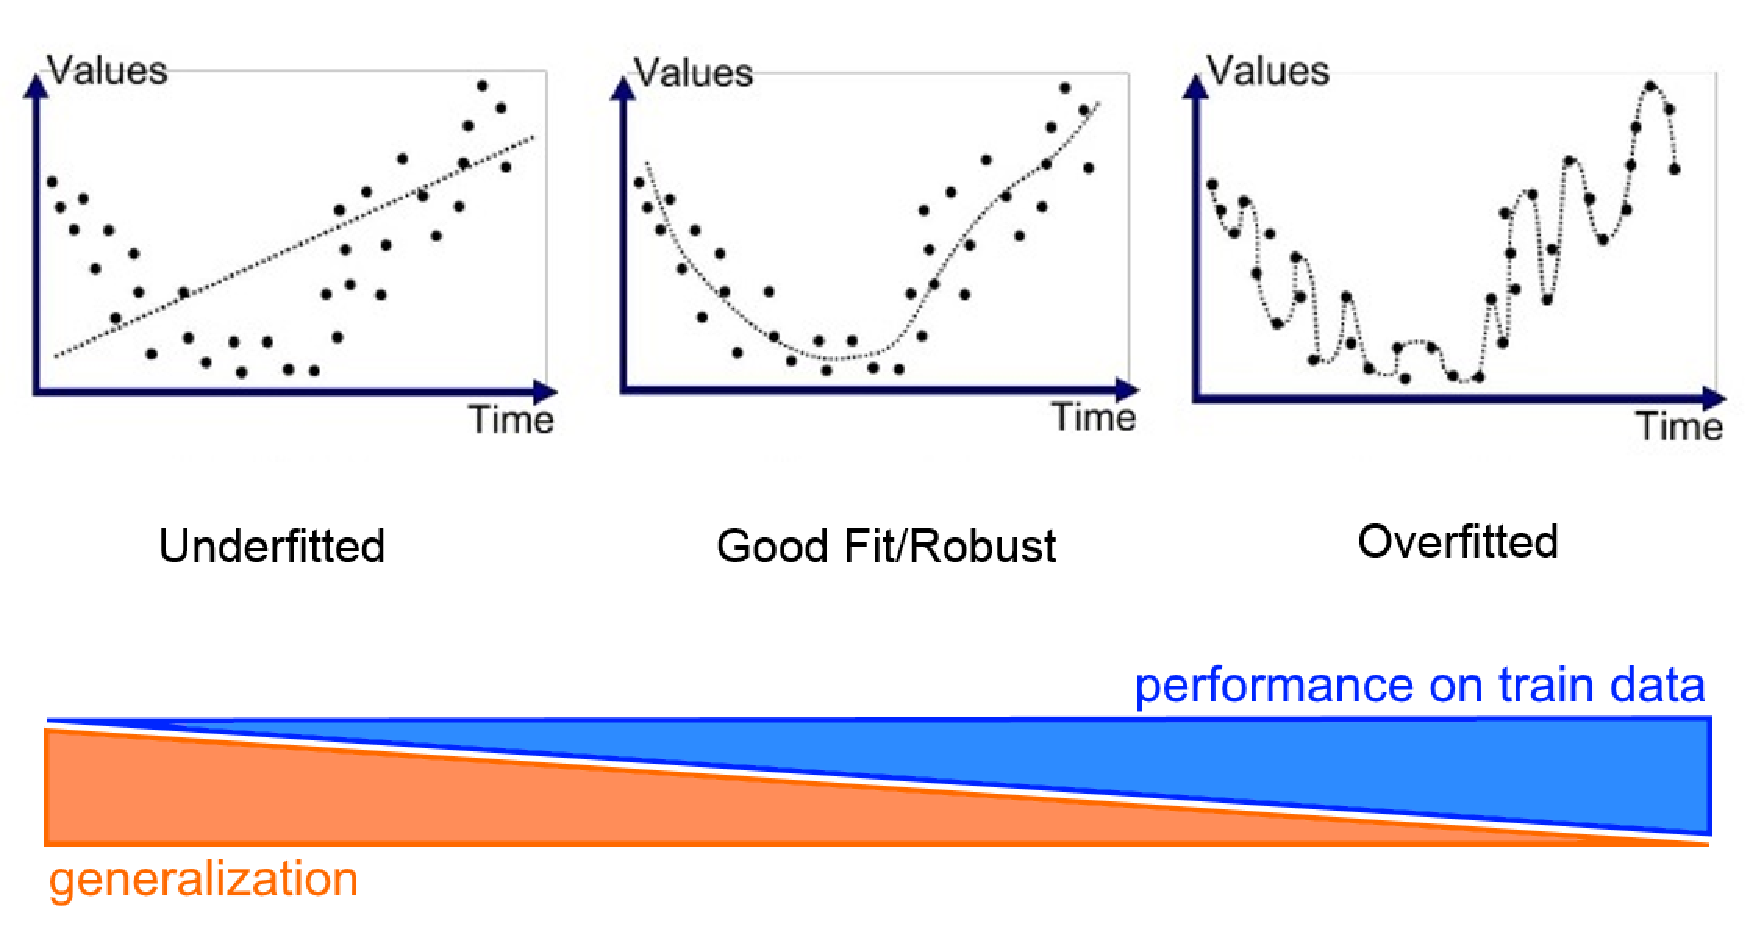
\includegraphics[width=\textwidth]{img/over_underfitting}
   \caption{Visualisation of under- and overfitting on a dataset.}
   \source{altered by the author, https://medium.com/greyatom/what-is-underfitting-and-overfitting-in-machine-learning-and-how-to-deal-with-it-6803a989c76, accessed: 29.03.2019}
   \label{fig:over_underfitting}
\end{figure}

Supervised learning on the other hand happens when the model is fed and trained upon example data with their correct classification labels present. The term 'supervised' therefore relates to the fact that presumably a human told the model which data points belong to which class. This approach is understandably more laborious because the creation of a labelled training's dataset takes time. The benefits are generally better performing models and the possibility to directly test the model. The testing is done by splitting the original training's dataset into two parts. Generally, a bigger portion ($\sim$ 75\%) is used for training the model and the other one ($\sim$ 25\%) - which the model has never seen during the fitting phase - is used to test the model's performance. \\
\newline
Frequently used terms in relation to ML are under- and overfitting. These terms correspond to two extremes of how the model and its incorporated (boundary-) function is fitted to the provided test-data (see points in figure \ref{fig:over_underfitting}). Underfitting describes the state, where the model does not seem to extract and comprehend any logic from the dataset and therefore over-generalises the classification or regression problem at hand (see outer left graph of figure \ref{fig:over_underfitting}). \\
The other extreme is known by the term overfitting where the model tries to correctly classify every single training-data point to its proper class. This results in the model being extremely tuned to the provided training-data but not being able to generalise well on new unseen data (see outer right graph in figure \ref{fig:over_underfitting}). In other words overfitting basically means that the model learned the training's data by hard which results in misleadingly high performance scores. The process of finding the balance between a model that is able to generalise on new data while identifying the underlying data-patterns is further described in section \ref{ml_text_data}.

\section{Ethics}

Drawing upon crowed sourced big-data is inevitably shadowed by ethical controversies. Using GPS locations and other sensitive data to identify and analyse patterns of human behaviour is rightfully criticised and sometimes considered unethical practise.\\
We are only talking about data that is publicly available, data that the user decided to share on the web on his or her own behalf - or is it?. The paper of \parencite{Estima2016} shows that not the entirety of data is voluntarily shared. Did the user sign up for his or her data to be systematically analysed? This depends on the Terms of Service (TOS) of the corresponding SMP which are hardly ever read by the consumer.\\
One has to understand the potential power this data possess. Having access to hundreds of personalised media objects of a specific social media user enables analytics to construct a blueprint of that person. This blueprint can encompasses the persons political orientation, its home and work location, preferences and dislikes as well as daily routines. Personalised advertisement would then be the smallest resulting threat. Interpersonal surveillance \parencite{Trottier2017}, stalking \parencite{Lyndon2011} or potential blackmailing through acquired sensitive information are by far greater and current threats. Additionally, it is unclear from a data-researcher point of view how to deal with encounters of media objects that indicate illegal behaviour e.g littering, assault or theft.\\

With that being said I personally think that the ethical discrepancy is legitimately continuously discussed in this context. Showing how the data and the anonymity of the authors is treated as well as the goal a project pursues are key elements that determine in my opinion if ethical terms are violated or not. 







\cleardoublepage
%\chapter{Working with \LaTeX\ }\label{sec:working}
This chapter explains how to typeset some of the most common elements contained in a technical report using \LaTeX.

\section{Headings}
Your report can be structured using several different types of headings. Use the commands \texttt{\textbackslash chapter\{.\}}, \texttt{\textbackslash section\{.\}}, \texttt{\textbackslash subsection\{.\}}, and \texttt{\textbackslash subsubsection\{.\}}. Use the asterisk symbol \texttt{*} to suppress numbering of a certain heading if necessary, for example, \texttt{\textbackslash section*\{.\}}.

\section{References and Footnotes}\label{sec:references}
References to literature are included using the command \texttt{\textbackslash
cite\{.\}}. For example \cite{optreg,motsys}. Your references must be entered in the file \texttt{bibliography.bib}. Making changes or adding new references in the bibliography file can be done manually or by using specialized software such as \textit{JabRef} which is free of charge.
 
Cross-referencing within the text is easily done using \texttt{\textbackslash label\{.\}} and \texttt{\textbackslash ref\{.\}}. For example, this paragraph is part of chapter~\ref{sec:working}; more specifically section~\ref{sec:references} on page~\pageref{sec:references}. You will need to compile your document twice in order for the cross-referencing to be updated.

Footnotes\footnote{The use of footnotes is generally not recommended.} are added using the command \texttt{\textbackslash footnote\{.\}}, but try to avoid the used of footnotes altogether.

\section{Lists}\label{sec:lists}
Three types of list-environments are commonly used: \texttt{itemize}, \texttt{enumerate}, and \texttt{description}. The following example uses \texttt{itemize} to create a list without numbering
\begin{itemize}
  \item point one; and
  \item point two
\end{itemize}
created using
\begin{verbatim}
\begin{itemize}
  \item point one; and
  \item point two
\end{itemize}
\end{verbatim}

The following example uses \texttt{enumerate} to create a list with numbering
\begin{enumerate}
  \item point one; and
  \item point two
\end{enumerate}
created using
\begin{verbatim}
\begin{enumerate}
  \item point one; and
  \item point two
\end{enumerate}
\end{verbatim}

The following example uses \texttt{description} to create a list with custom text as bullet-points
\begin{description}
  \item[P1] point one; and
  \item[P2] point two
\end{description}
created using
\begin{verbatim}
\begin{description}
  \item[P1] point one; and
  \item[P2] point two
\end{description}
\end{verbatim}


\section{Tables}\label{sec:tables}
Table~\ref{tab:table} shows an example of a simple table-layout. Try to avoid vertical lines on tables. The Internet contains countless resources on how to create special elements and structures in tables such as cells spanning multiple rows, rotated text, sideways tables, justification of cell elements, etc.
\begin{table}[ht]
\begin{center}
\caption{Driving cycle data of ECE-15, EUDC, and NEDC.}\vspace{1ex}
\label{tab:table}
\begin{tabular}{llccc}\hline
Description & Unit & ECE & EUDC & NEDC \\ \hline
Duration & s & 780 & 400 & 1180 \\
Distance & km & 4.052 & 6.955 & 11.007 \\
Average velocity & km/h & 18.7 &  62.6 & 33.6 \\
Idle speed & \% & 36 & 10 & 27 \\ \hline
\end{tabular}
\end{center}
\end{table}

This table was created using
\begin{verbatim}
\begin{table}[ht]
\begin{center}
\caption{Driving cycle data of ECE-15, EUDC, and NEDC.}\vspace{1ex}
\label{tab:table}
\begin{tabular}{llccc}\hline
Description & Unit & ECE & EUDC & NEDC \\ \hline
Duration & s & 780 & 400 & 1180 \\
Distance & km & 4.052 & 6.955 & 11.007 \\
Average velocity & km/h & 18.7 &  62.6 & 33.6 \\
Idle speed & \% & 36 & 10 & 27 \\ \hline
\end{tabular}
\end{center}
\end{table}
\end{verbatim}
Table~\ref{tab:table_advanced} shows a more advanced version of Tab.~\ref{tab:table} using the \texttt{booktabs} package. Inspect the source code of this document to see how this was done.
\begin{table}[ht]
\begin{center}
\small
\caption{Driving cycle data of ECE-15, EUDC, and NEDC.}\vspace{1ex}
\label{tab:table_advanced}
\begin{tabular}{@{}lcccc@{}}\toprule[1.5pt]
& & \multicolumn{3}{c}{\bf Driving cycle}\\
\cmidrule{3-5}
Description & Unit & {ECE} & {EUDC} & {NEDC} \\ \midrule
Duration & \unit[]{s} & 780 & 400 & 1180 \\
Distance & \unit[]{km} & 4.052 & 6.955 & 11.007 \\
Average velocity & \unitfrac[]{km}{h} & 18.7 &  62.6 & 33.6 \\
Idle speed & \unit[]{\%} & 36 & 10 & 27 \\ \bottomrule[1.5pt]
\end{tabular}
\end{center}
\end{table}



\section{Working with Units}
The package \texttt{\textbackslash usepackage\{units\}} enables two useful commands, namely \texttt{\textbackslash unit[.]\{.\}} and \\ \texttt{\textbackslash unitfrac[.]\{.\}\{.\}}. Use these commands to display units in a concise way, for example
\begin{align}
\delta t &= \unit[1]{s}\\
v &= \unitfrac[5]{m}{s}.
\end{align}
This example was done using
\begin{verbatim}
\begin{align}
\delta t &= \unit[1]{s}\\
v &= \unitfrac[5]{m}{s}.
\end{align}
\end{verbatim}

\section{Including Graphics}\label{sec:epsgraph}
It is recommended that you only use encapsulated post-script graphics \texttt{.eps} in your report. If you mix \texttt{.eps} with other formats such as \texttt{.png}, \texttt{.jpeg} or \texttt{.gif}, you will most likely not be able to compile your report without errors. Note that figures created in \textsc{Matlab} are easily saved in \texttt{.eps} format.

The inclusion of a figure can be done in the following way:
\begin{verbatim}
\begin{figure}[ht]
   \centering
   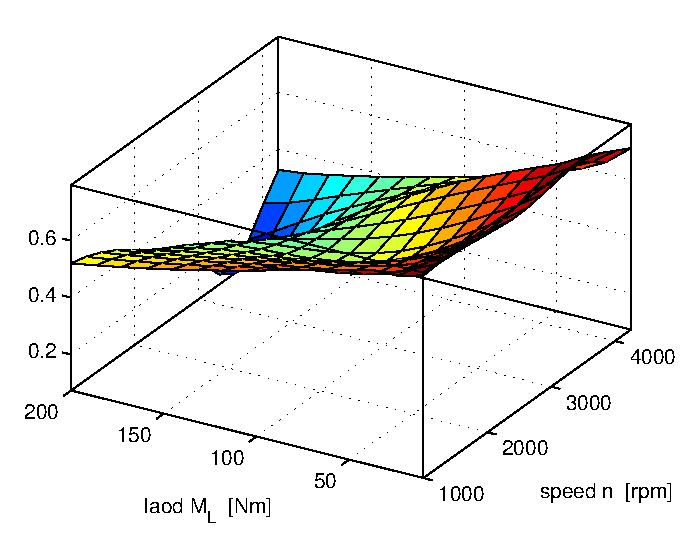
\includegraphics[width=0.75\textwidth]{img/k_surf.eps}
   \caption{Example of a figure.}
   \label{img:k_surf}
\end{figure}
\end{verbatim}

\begin{figure}[ht]
   \centering
   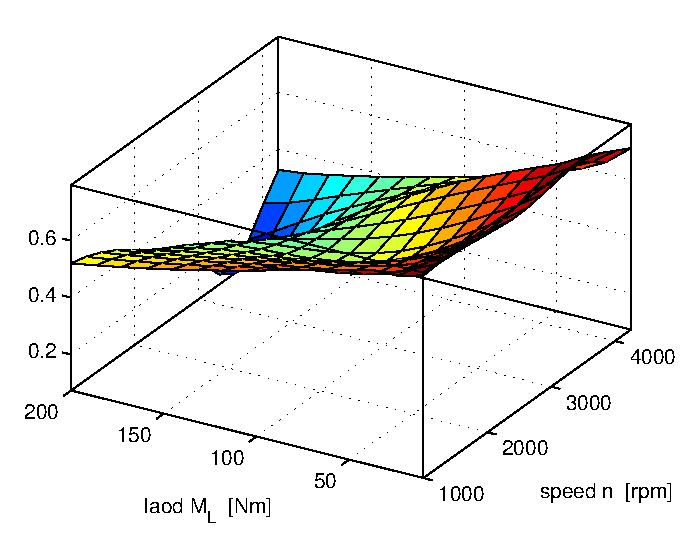
\includegraphics[width=0.75\textwidth]{img/k_surf.eps}
   \caption{Example of a figure.}
   \label{img:k_surf}
\end{figure}

Two figures are displayed next to each other using
\begin{verbatim}
\begin{figure}[ht]
  \begin{minipage}[t]{0.48\textwidth}
    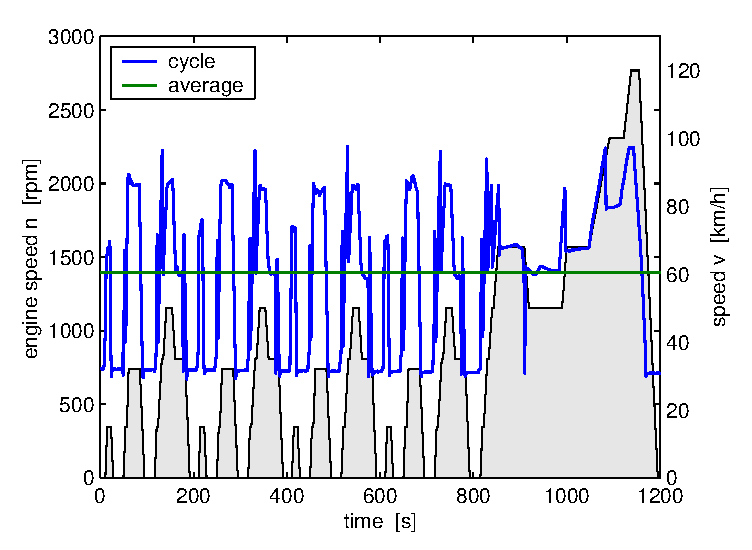
\includegraphics[width = \textwidth]{img/cycle_we.eps}
  \end{minipage}
  \hfill
  \begin{minipage}[t]{0.48\textwidth}
    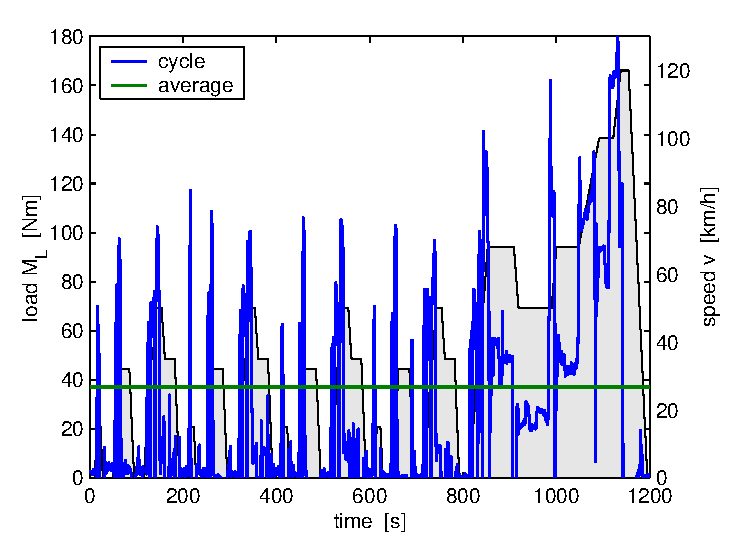
\includegraphics[width = \textwidth]{img/cycle_ml.eps}
  \end{minipage}
  \caption{Two figures next to each other.}
  \label{img:cycle}
\end{figure}
\end{verbatim}

\begin{figure}[ht]
  \begin{minipage}[t]{0.48\textwidth}
    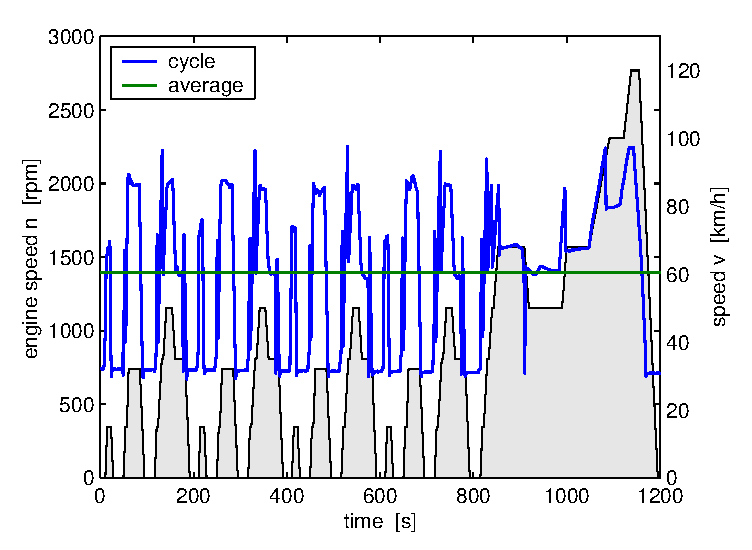
\includegraphics[width = \textwidth]{img/cycle_we.eps}
  \end{minipage}
  \hfill
  \begin{minipage}[t]{0.48\textwidth}
    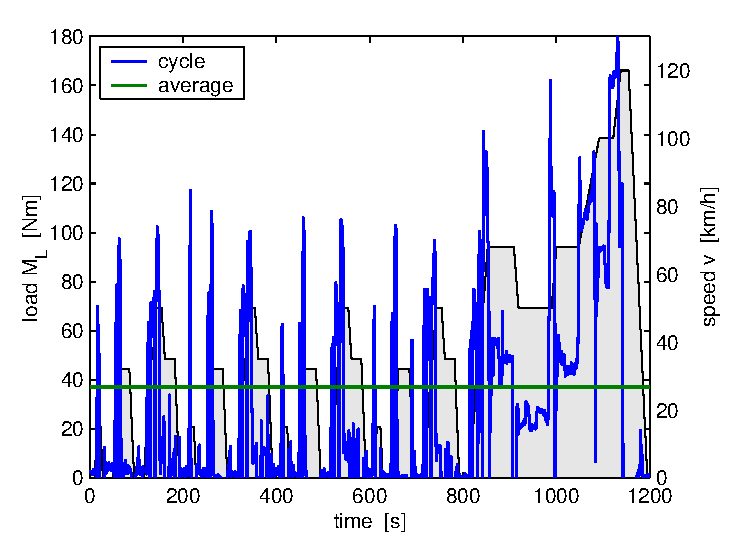
\includegraphics[width = \textwidth]{img/cycle_ml.eps}
  \end{minipage}
  \caption{Two figures next to each other.}
  \label{img:cycle}
\end{figure}

The positioning parameter \texttt{h} (here) forces your figure to be placed in the current position relative to your text. You may add \texttt{t} (top), \texttt{b} (bottom), and/or \texttt{p} (page) to allow for more flexible positioning within your document. For instance, \texttt{[tb]} forces your figure to be placed either on the top or bottom of a page.


\section{Equations}\label{sec:math}
The most common way to include equations is using the \texttt{equation} environment.
\begin{equation}\label{eq:p_me0f}
 p_\mathrm{me0f}(T_e,\omega_e) \ = \ k_1(T_e) \cdot (k_2+k_3 S^2
 \omega_e^2) \cdot \Pi_\mathrm{max} \cdot \sqrt{\frac{k_4}{B}} \, .
\end{equation}
It is recommended to use \texttt{\textbackslash mathrm\{.\}} for subscripts comprising more than two letters since it reduces the width of the subscript significantly and improves readability. The corresponding code is
\begin{verbatim}
\begin{equation}\label{eq:p_me0f}
 p_\mathrm{me0f}(T_e,\omega_e) \ = \ k_1(T_e) \cdot (k_2+k_3 S^2
 \omega_e^2) \cdot \Pi_\mathrm{max} \cdot \sqrt{\frac{k_4}{B}} \, .
\end{equation}
\end{verbatim}
Equations, such as Eq.~\eqref{eq:p_me0f}, may be referenced using \texttt{\textbackslash eqref\{.\}}. In-line mathematical content is created using \texttt{\$.\$}, for example $a^2+b^2=c^2$. It is practically possible to typeset any equation in \LaTeX. Equation~\eqref{eq:advanced} shows an example of a more advance structure.
\begin{equation}\label{eq:advanced}
x^k_n(i) = \left\{\begin{array}{ll}y(i) & \text{if}\quad x^k_{n-1}(i)\leq \mathbf{x}\\
z(i) & \text{otherwise}\end{array}\right., \text{for}\quad i=\{1,\ldots,N\}.
\end{equation}



\section{Including Code in your Document}
Include samples from your Matlab code using the \texttt{lstlistings} environment, for example
\lstset{language=Matlab,numbers=none}
\begin{lstlisting}[frame=lines]
% Evaluate y = 2x
for i = 1:length(x)

  y(i) = 2*x(i);

end
\end{lstlisting}
This example was created using
\begin{verbatim}
\lstset{language=Matlab,numbers=none}
\begin{lstlisting}[frame=lines]
% Evaluate y = 2x
for i = 1:length(x)

  y(i) = 2*x(i);

end
\end{lstlisting}
\end{verbatim}
where \texttt{\textbackslash usepackage\{mcode\}} must be included in the preamble of your document. If you want to include the entire content of a file \texttt{mycode.m} in your document, simply input the path to \texttt{mycode.m} instead of pasting the entire content into your \TeX -file
\begin{verbatim}
\lstset{language=Matlab,numbers=left}
\lstinputlisting{path/to/mycode.m}
\end{verbatim}
Including the path to your m-file also ensures that the code in your report is always up-to-date. The \texttt{\textbackslash lstset\{language=Matlab\}} command ensures that \textsc{Matlab} syntax definitions are used, but many other languages are recognised as well such as \texttt{Fortran} and \texttt{C++}.

\cleardoublepage
% \input{}
% \cleardoublepage
% \input{}
% \cleardoublepage
% ...
\chapter*{Used Software}\addcontentsline{toc}{chapter}{Used Software}

\section*{Programming:}
\begin{large}Scripting language\end{large}
\begin{tabbing}
 \hspace*{5cm}  \= \kill
 Python \> v.3.6.7
\end{tabbing}
\textbf{Used libraries:}\\
\newline
\begin{large}Data-management\end{large}
\begin{tabbing}
 \hspace*{5cm}  \= \kill
 psycopg2 \> v.2.7.7 \\
 pandas \> v.0.24.1 \\
 numpy \> v.1.16.1
 \end{tabbing}
\begin{large}Plots and graphs\end{large}
\begin{tabbing}
  \hspace*{5cm}  \= \kill
  matplotlib \> v.3.0.2 \\
  mglearn \> v.0.1.7
 \end{tabbing}
\begin{large}Machine learning\end{large}
 \begin{tabbing}
  \hspace*{5cm}  \= \kill
  scikit-learn \> v.0.20.2 \\
  joblib \> v.0.13.1
 \end{tabbing}
\begin{large}Text-processing\end{large}
 \begin{tabbing}
  \hspace*{5cm}  \= \kill
   nltk \> v.3.4 \\
   pyenchant \> v.2.0.0
  \end{tabbing}
 \begin{large}Application Program Interfaces (APIs)\end{large}
 \begin{tabbing}
  \hspace*{5cm}  \= \kill
  google-cloud \> v.0.34.0 \\
  google-cloud-vision \> v.0.35.2 \\
  flickrapi \> v.2.4.0 \\
  geocoder \> v.1.38.1
 \end{tabbing}
\begin{large}Web-crawling and HTML handling\end{large}
 \begin{tabbing}
  \hspace*{5cm}  \= \kill
   bs4 \> v.0.0.1 \\
   urllib3 \> v.1.24.1 \\
 \end{tabbing}
 
 \section*{Geographic Information System (GIS):}
  \begin{tabbing}
  \hspace*{5cm}  \= \kill
   QGIS \> v.3.4.4
 \end{tabbing}
 \section*{Relational Database Management System (RDM):}
  \begin{tabbing}
  \hspace*{5cm}  \= \kill
   PostgrSQL \> v.11.1 \\
   pgAdmin4 \> v.3.5
 \end{tabbing}
 
 \section*{Image editing software:}
  \begin{tabbing}
  \hspace*{5cm}  \= \kill
   Paint.NET \> v.4.1.5
 \end{tabbing}

 
 
 
 
 
 
 
 
 
 
 
 
 
 
 
 


% Appendix______________________________________________________________________
\appendix
\appendix

\chapter{Code} \label{python_code}

\chapter{SQL queries for training data} \label{sql_queries_for_trainingdata}

%\chapter{Confusion matrix} \label{confusion_matrix}

\chapter{Model validation tables} \label{model_validation_tables}

\chapter{Best M2 class-features} \label{M2_top_features}

\chapter{Interview templates} \label{interview_templates}

\chapter{Passive observation templates} \label{passive_obs_templates}




% Bibliography__________________________________________________________________
% Literature (Additional references can be added to the .bib-file manually, or by using, for example, the free application JabRef). Compile in the following order: latex -bibtex -latex -latex

\bibliographystyle{plain}
\bibliography{bibliography}

\end{document}
